
\documentclass[conference]{IEEEtran}
\usepackage{color}

% *** MISC UTILITY PACKAGES ***
%
%\usepackage{ifpdf}
% Heiko Oberdiek's ifpdf.sty is very useful if you need conditional
% compilation based on whether the output is pdf or dvi.
% usage:
% \ifpdf
%   % pdf code
% \else
%   % dvi code
% \fi
% The latest version of ifpdf.sty can be obtained from:
% http://www.ctan.org/tex-archive/macros/latex/contrib/oberdiek/
% Also, note that IEEEtran.cls V1.7 and later provides a builtin
% \ifCLASSINFOpdf conditional that works the same way.
% When switching from latex to pdflatex and vice-versa, the compiler may
% have to be run twice to clear warning/error messages.

\usepackage{cite}
% cite.sty was written by Donald Arseneau
% V1.6 and later of IEEEtran pre-defines the format of the cite.sty package
% \cite{} output to follow that of IEEE. Loading the cite package will
% result in citation numbers being automatically sorted and properly
% "compressed/ranged". e.g., [1], [9], [2], [7], [5], [6] without using
% cite.sty will become [1], [2], [5]--[7], [9] using cite.sty. cite.sty's
% \cite will automatically add leading space, if needed. Use cite.sty's
% noadjust option (cite.sty V3.8 and later) if you want to turn this off.
% cite.sty is already installed on most LaTeX systems. Be sure and use
% version 4.0 (2003-05-27) and later if using hyperref.sty. cite.sty does
% not currently provide for hyperlinked citations.
% The latest version can be obtained at:
% http://www.ctan.org/tex-archive/macros/latex/contrib/cite/
% The documentation is contained in the cite.sty file itself.

\usepackage{hyperref}



% *** GRAPHICS RELATED PACKAGES ***
%
\ifCLASSINFOpdf
  \usepackage[pdftex]{graphicx}
  % declare the path(s) where your graphic files are
  % \graphicspath{{../pdf/}{../jpeg/}}
  % and their extensions so you won't have to specify these with
  % every instance of \includegraphics
  \DeclareGraphicsExtensions{.pdf,.jpeg,.png}
\else
  % or other class option (dvipsone, dvipdf, if not using dvips). graphicx
  % will default to the driver specified in the system graphics.cfg if no
  % driver is specified.
  % \usepackage[dvips]{graphicx}
  % declare the path(s) where your graphic files are
  % \graphicspath{{../eps/}}
  % and their extensions so you won't have to specify these with
  % every instance of \includegraphics
  % \DeclareGraphicsExtensions{.eps}
\fi
% graphicx was written by David Carlisle and Sebastian Rahtz. It is
% required if you want graphics, photos, etc. graphicx.sty is already
% installed on most LaTeX systems. The latest version and documentation can
% be obtained at:
% http://www.ctan.org/tex-archive/macros/latex/required/graphics/
% Another good source of documentation is "Using Imported Graphics in
% LaTeX2e" by Keith Reckdahl which can be found as epslatex.ps or
% epslatex.pdf at: http://www.ctan.org/tex-archive/info/
%
% latex, and pdflatex in dvi mode, support graphics in encapsulated
% postscript (.eps) format. pdflatex in pdf mode supports graphics
% in .pdf, .jpeg, .png and .mps (metapost) formats. Users should ensure
% that all non-photo figures use a vector format (.eps, .pdf, .mps) and
% not a bitmapped formats (.jpeg, .png). IEEE frowns on bitmapped formats
% which can result in "jaggedy"/blurry rendering of lines and letters as
% well as large increases in file sizes.
%
% You can find documentation about the pdfTeX application at:
% http://www.tug.org/applications/pdftex





% *** MATH PACKAGES ***
%
\usepackage[cmex10]{amsmath}
% A popular package from the American Mathematical Society that provides
% many useful and powerful commands for dealing with mathematics. If using
% it, be sure to load this package with the cmex10 option to ensure that
% only type 1 fonts will utilized at all point sizes. Without this option,
% it is possible that some math symbols, particularly those within
% footnotes, will be rendered in bitmap form which will result in a
% document that can not be IEEE Xplore compliant!
%
% Also, note that the amsmath package sets \interdisplaylinepenalty to 10000
% thus preventing page breaks from occurring within multiline equations. Use:
\interdisplaylinepenalty=2500
% after loading amsmath to restore such page breaks as IEEEtran.cls normally
% does. amsmath.sty is already installed on most LaTeX systems. The latest
% version and documentation can be obtained at:
% http://www.ctan.org/tex-archive/macros/latex/required/amslatex/math/










\usepackage[font=footnotesize,labelsep=period]{caption}
\renewcommand{\figurename}{Figure}
%\usepackage[font=footnotesize]{subfig}
% subfig.sty, also written by Steven Douglas Cochran, is the modern
% replacement for subfigure.sty. However, subfig.sty requires and
% automatically loads Axel Sommerfeldt's caption.sty which will override
% IEEEtran.cls handling of captions and this will result in nonIEEE style
% figure/table captions. To prevent this problem, be sure and preload
% caption.sty with its "caption=false" package option. This is will preserve
% IEEEtran.cls handing of captions. Version 1.3 (2005/06/28) and later
% (recommended due to many improvements over 1.2) of subfig.sty supports
% the caption=false option directly:
%\usepackage[caption=false,font=footnotesize]{subfig}
%
% The latest version and documentation can be obtained at:
% http://www.ctan.org/tex-archive/macros/latex/contrib/subfig/
% The latest version and documentation of caption.sty can be obtained at:
% http://www.ctan.org/tex-archive/macros/latex/contrib/caption/

\usepackage{fixltx2e}
\usepackage{stfloats}

%\usepackage{url}


% correct bad hyphenation here
\hyphenation{op-tical net-works semi-conduc-tor}

\usepackage{xcolor}

\colorlet{pcolor}{blue}
\colorlet{fcolor}{red}
\newcommand{\e}[2][fcolor]{\textcolor{pcolor}{[}\textcolor{#1}{#2}\textcolor{pcolor}{]}}

\hypersetup{
    bookmarks=true,         % show bookmarks bar?
    unicode=true,           % non-Latin characters in Acrobat’s bookmarks
    pdftoolbar=true,        % show Acrobat’s toolbar?
    pdfmenubar=true,        % show Acrobat’s menu?
    pdffitwindow=false,     % window fit to page when opened
    pdfstartview={FitH},    % fits the width of the page to the window
    pdftitle={An Ontology Polysystem Driven Technique for Semantic Markup
  for Edited Documents},    % title
    pdfauthor={Evgeny Cherkashin, Kristina Paskal, Igor Bychkov,
      Polina Belykh},     % author
    pdfsubject={Scientific paper},   % subject of the document
    pdfcreator={LaTeX},   % creator of the document
    pdfproducer={LaTeX}, % producer of the document
    pdfkeywords={polysystem} {ontology} {semantic web} {knowledge
      acquisition} {data mining} {natural language processing}, % list of keywords
    pdfnewwindow=true,      % links in new window
    colorlinks=true,       % false: boxed links; true: colored links
    %linkcolor=[rgb]{0 0.4 0.1},          % color of internal links (black)
    linkcolor=black,          % color of internal links (black)
    citecolor=blue,        % color of links to bibliography
    filecolor=black,      % color of file links
    %urlcolor=[rgb]{0.3 0.0 0.3}           % color of external links
    urlcolor=black           % color of external links
}


\begin{document}
\title{An Ontology Polysystem Driven Technique for Semantic Markup for
  Edited Documents} \author{\IEEEauthorblockN{Evgeny
    Cherkashin\IEEEauthorrefmark{1}\IEEEauthorrefmark{2}\IEEEauthorrefmark{3},
    Kristina Paskal\IEEEauthorrefmark{2}\IEEEauthorrefmark{3}, Igor
    Bychkov\IEEEauthorrefmark{1}, Polina Belykh\IEEEauthorrefmark{1}}%
  \IEEEauthorblockA{\IEEEauthorrefmark{1}Institute of System Dynamics
    and Control Theory at SB RAS, Irkutsk, Lermontov str., 134,
    664033, Russia}%
  \IEEEauthorblockA{\IEEEauthorrefmark{2}National Research Irkutsk
    State Technical University, Irkutsk, Lermontov str., 83, 664074,
    Russia}%
  \IEEEauthorblockA{\IEEEauthorrefmark{3}Irkutsk State University,
    Irkutsk, Gagarina blvd., 664003, Russia}%
\texttt{\small eugeneai@icc.ru}
}

% use for special paper notices
%\IEEEspecialpapernotice{(Invited Paper)}

% make the title area
\maketitle


\begin{abstract}
  A general idea of an approach to representation and induction of a
  semantic markup (logical layer) for description of the text content
  (e.g., internet sites and legal documents) is being described.  The
  logical layer is being generated on the base of analysis of changes
  introduced by user.  The changes of the text and the logical layer
  are analyzed.  The variant of the interpretation of the changes,
  e.g., error correction of a value or a new statement definition, is
  determined by means of user interview.  The theoretical basis of the
  technique is the usage of a polysystem representation of ontologies
  for the domain.  The presentation is a hierarchically fibered
  structure of concepts and relations, which are mapped between fibers
  by means of interpretation relations.

  An automation of document preparation activities in a notary office
  has been chosen as a testing ground for approbation of the
  technologies under development.  The documents that are originated
  and used there contain information represented as structural and
  nonstructural data equally likely.
\end{abstract}


% For peer review papers, you can put extra information on the cover
% page as needed:
% \ifCLASSOPTIONpeerreview
% \begin{center} \bfseries EDICS Category: 3-BBND \end{center}
% \fi
%
% For peerreview papers, this IEEEtran command inserts a page break and
% creates the second title. It will be ignored for other modes.
\IEEEpeerreviewmaketitle



\section{Introduction}
% no \IEEEPARstart
In 2001 Tim Berners-Lee proposed a blueprint \cite{TBL2001} of web
development that is aimed at the implementation of network services
with reasonable integration of logical layer of the information
presented.  The information was to be marked up semantically and the
program agents where to take advantage of the markup as the logical
layer for the information consumption and processing.  The blueprint
is called Semantic Web.

One of the main problems of SW is the fact, that the regular users of
web resources are not fond of the complex technological aspects of SW.
They are interested in their practical problems solutions.  In order
to involve users in SW content development, that aspects must be
completely hidden.  This results in the necessity of development of
document and site content management software exploited within SW as
knowledge acquisition systems, where user has to play role of
information source for a system-integrated decision-making engine
inducing formal knowledge on the base of data analysis.

To be more comprehensible consider a content of a legal document,
which in most cases contains meaningful information on human beings
relationships that is usually passed to other documents in a
derivative form.  This suggests an idea to develop a form of the
logical layer representation in a reasonably detailed form, which can
be rendered as a regular text pages by means of context-depended (in
sense of a legal document) text templates.  The SW approach could
supplement the idea with data formats and technologies of their
storage and processing.  SW represents logical layer as a network graph
of notions and relations between the notions.  For example, individuals
mentioned in a legal document relate to the document as
“part-whole”, unless to speak even more explicitly in a context of
the meaningful information.

At present most of the use cases of domain ontology models are
refining search results.  Automatic procedures of ontology extraction
from the documents are based on crawling documents in a warehouse,
running data mining procedures on the text content and metadata
attributes of the documents.  Simple observation of the human behavior
in the process of a document preparation will result in the confidence
that meaningful parts of the document, which are usually expressed
with the logical layer, are located at the points of document changes.
Hence, a programming system automating a document preparation should
track the changes and analyze them in time to extract ontology structure,
i.e., objects, concepts and relation between them.

The logical layer is induced during content edition by means of data
mining and user interview.  The context of the knowledge acquisition
consists of a polysystem \cite{father} of ontologies describing the
domain, the source document (its text representation and the existing
logical structure), its list of modifications in a transaction, user's
action history, and answers to the interview questions clarifying
meaning of text content changes and properties of the relations
constructed.  As a result, new or modified triples \texttt{<subject,
  relation, object>} representing the domain are constructed.
Collected triple data, metadata and knowledge of the logical layer can
also be crawled on a regular basis to figure out patterns and
functional relations between attributes (triple's objects).  In the
last case a relational table could be induced to rise the efficiency
of data storage and processing.

The present trends of internet information system development show
that the systems become a web-services and are oriented to support
social networks \cite{SN}.  The data flow processing there in most
cases is input, storage, filtering and transmitting data, i.e., the
social networks integrate rather than aggregate data, e.g., to produce
reports.  Hence, the usage of special design techniques for the
middle-ware layer of the software, such as object-oriented design, is
not a significant technological advantage.  Social network nodes are
interconnected with standardized protocols and data structures, and
has the same way of integration with other social networks.

Let us emphasize the properties of social network software:
\begin{IEEEitemize}[\IEEEsetlabelwidth{Z}]
\item there are no predominant common global task to be solved by
  agents (computer and human) of the SN;
\item each agent solves its special task acquiring data from other
  data sources and agents, hence, the agent's APIs’ and
  supported data format must be standardized;
\item human users of the social network do most of the aggregation
  tasks personally including subconscious joint processing of
  unstructured and semantic information;
\item a good practice is to use cheap virtual hosting to run the
  a SW node, therefore, the information system itself must be written
  according to the restrictions of a server-side programming language,
  like PHP, and utilize the computational and data storage resources
  of client workstation and its browser environment.
\end{IEEEitemize}

In this paper, we continue the development of the approach
\cite{prevwork} to document and site content management and
integration within a general study \cite{b2:15}, and briefly consider
the procedure of polysystem ontology usage in the process of user
dialog maintenance.

\section{Document Markup}

Resource description framework (RDF) standard describes informational
resources with triples \texttt{<subject, relation, object>} in a
context.  A set of triples forms a graph (network) of data and
relations reflecting knowledge.  It is convenient to divide graphs to
subgraphs and construct hierarchic complexes \cite{b2:15}, resulting a
hierarchy of contexts.  In a general case, a context affects the
interpretation of the set of triples coupled with it.  For example, in
a legal notary document family name and passport data are presented as
texts in different parts of the document, but they related to the
single person in the context defined by the document.  So the parts of
the document form the contexts of text rendering for the passport
data.

The rendering engine we considered in \cite{prevwork}.  According to
this approach, all the template data for document rendering is also
stored in the ontology graph.  We also represent the views and
algorithms implementing controllers in the sense of MVC (Model View
Controller) \cite{b2:5} technique with triples \cite{b5}.  The content
of the document from a general view is a tree, where almost each node
is both a subject and an object of their corresponding relations.  The
root node can be only a subject, and the leaf nodes are objects only.
In the higher level hierarchies, e.g. in a tree of the documents in a
warehouse, the root node is an object node as well\,: it is referred
from a record of the warehouse.

\section{Document Markup Scheme}
\label{sec:scheme}

The proposed way of semantic document markup is to track and interpret
the results of document editing.  Let's suppose that a document body
change affects the meaning of the document, hence, alters its logical
layer.  The following trivial modifications that are the elementary
error correction are not considered to be a valuable information for
the markup: a field value change (an object of a triple), paragraph
text editing that might imply its origin template correction.  The
changes of our interest result in a new triple relation construction
between context subjects and old/new object value.  The text change
analysis is aimed at data and knowledge acquisition, where the content
management system plays an active role, and user is a source of
complementary information.

The first question that user have to be asked is to determine weather
a change is an above mentioned trivial one.  If it is not, then the
semantic layer enrichment procedure is carried on.  The source of data
to decision-making procedure of a triple formation/modification is an
environment containing a) logic information (thanks to the previous
version of document is already supplied with a logical layer); b) the
source version of the document, c) a text modification expressed in
diff format \cite{b9}; d) user answers to the question asked by the
system, refining the semantics and structure of the modifications; e)
user actions preceding the modification.  The list of the previous
user's actions can reveal a general intention, e.g., if user made a
copy of document and changed an individual name, this would imply the
necessity to fill in the passport data, which, in turn, implies
filling in a number of triples with new values representing the new
individual (subject) of the document.

At the firs step the extent of the modified value is determined.  It
could be a word, a phrase, a sentence, the whole object value, or an
extent of a text markup (e.g. HTML tag value).  The variant is
specified by user.

The simplest way of the triple formation procedure is to allow the
user to choose subject and relation from list of all relevant subjects
mentioned in the document and their relations and construct a new
triple \texttt{<subject,relation,old object>}.  The list of subjects
is constructed from a tree of all the subjects of the edited document
and the edited object itself.  After the first choice is made, a list
of all available relation is constructed from all known relation of
the chosen subject, its class and parent classes.  User must choose
one relation to form the triple.  In the case, when the list contains
no adequate relation, a new one must be defined.  New relation is
always a subclass of one that already exists in the system, which is
also chosen from the list.  New relations defined by inexperienced user
must be periodically analyzed by knowledge engineers to get rid of
semantic inaccuracy, contradictions, redundancy to the equivalents,
and be, hence, refactored.

If a value of a triple is removed, then the triple is to be removed
too.  The situation is acceptable if the minimal structural and
semantic completeness of all the subjects of the documents holds,
otherwise either the user delete action is prohibited or the chain
recursive deletion of the subjects is initiated.  To control this
behavior each subject class have to be accompanied with a list of
minimal valuable triplets that define the basis of the subject
meaning.  Partial text removal, if it is not an error correction, is
processed analogously to modification, with removed part being the
object value.  Addition of characters to text is an action similar to
modification, i.e., in a general case a new triple is constructed.

Addition of a triple might result in extending the document with new
subjects and relations.  For example, let construct a new tripartite
agreement from an existing bilateral one.  In the new agreement the
third individual appears, so the addition of a new family name of the
individual results in construction of a subject for the individual,
filling in the necessary triples, as well as definition of a new
relation between document and the third individual as a subclass of
\texttt{structuralElement:} relation.  This stage is necessary as all
new subjects must be in a relation with other ones.

\section{Theoretical Generalization of the Acquisition Process}

The above described approach is a simplified step-wise implementation
of the procedure of polysystem analysis and synthesis \cite{father}
(PPAS).  This is a general procedure for system analysis of domains.
The essence of the approach is that domain and any its object or
process can be fibrated and represented in multidimensional space of
fiber-coordinates.  The fiber consists of concepts and morphisms
between them.  This approach is used in decomposition, analysis and
synthesis of complex systems.  For each concepts of a fiber there
exists another concept in different fiber, which is identical to the
former concept via an interpretation.  All the concepts are
interpreted by concepts of the abstract system fiber.  The same is
true for the morphisms.  In comparison to system approach, where the
principle of interconnection of the elements is fundamental,
polysystem analysis assumes the hypothesis of fibration, i.e., it
supposes a possibility of representation of the object under
investigation as disjoint fibers, thus, mutually unbound fibers
(subdomains).  So, in a generalized insight a polysystem is a system
itself, and polysystem analysis is a new form of system analysis.

According to PPAS \cite{father} each concept of an aspect should be
presented (via interpretation morphisms) in all other fibers as well
as its relationships with adjacent concepts.  For each of the fibers,
a complete theory of the domain can be constructed.  Each theory
differ by their fundamental concept, but they are similar each other
via concept substitution via interpretation.  This allows us to induce
new axiomatic theories of domains in the image and likeness of the
known ones.  Each system domain (fiber) of knowledge fibrates multiply
and sequentially, giving raise of the polysystem of representation of
an object under investigation.  All the system theories are combined
in the unified model describing the domain and the object.

The application of the PPAS to the process of data and knowledge
acquisition in the documents expressed as simultaneus polysystem
fibering the domain in various coordinate systems (aspects) as
follows\,: structural organization of a document (mereological
aspect), expressing domain of activity area, hierarchical inheritance
of various kind of documents (domain system concept inheritance),
people and organization relationship, deontic logic representation of
the document meaning, etc.  Having established new class or new
relation between two classes, the concept or relation should be
reflected as a substituted (interpreted with) one in other ontologies
(e.g., mereological one).  To make the polysystem be easily
understandable we must also produce the definitions for the concepts
in a natural language in terms of those ontologies.  The requirement
of belonging an object to a class, inheritance between classes and
relations reflects the idea of hierarchical polysystem fibering and
are the examples of implementation of concept interpretations between
the fibers.

Thus, the usage of the PPAS allows us to a) control the completeness
of the system of objects in a document with respect to their
interpretation to a predefined abstract system fiber, which we roughly
call ``template fiber''; b) verify the soundness with respect to the
semantics of the relation defined again via interpretations; and in a
distant future c) automatically produce program implementing the fiber
theories via interpretation of the existing algorithms on other
fibers.  In Russian literature the notion ``fiber'' usually referred
to as ``layer''.  In the rest of the paper we will sometimes use word
layer as synonym to fiber.

\section{Maintaining a Dialogue With User}

The through interpretation feature of polysystem layers could be used
to maintain user interview dialog on the base of an inference by
analogy represented as movement along relations, morphisms and
interpretation in the polysystem of ontologies.

In order to realize the dialog procedure, there should already exist
fibers representing ``part-whole'' relations, class hierarchies of the
abstract concepts, correspondence of objects to classes, set theories
and necessary domain layers, e.g., the fiber defining that men and
women are disjoint concepts.  The aim of the user dialog is to define
that the object belongs to a context (fiber), determine its
interpretations into concepts of other fibers, and to provide all the
context to be complete with respect to their template fibers.  The
dialog is maintained on the base of analysis of known properties and
restrictions (relations) of the subject\,: type of data representing
the subject, its location in the context hierarchy, existing relations
with other subjects and objects, etc.

Let's consider simple family relationships in fig.~\ref{OPSA}, where
most of the obvious relations are hidden to make the figure more
readable.  There are a part o the domain polysystem including four
main layers, which model various aspects of Bob's family: layer 1
represents the family itself, it is the only layer having objects as
concepts; layer 2 represent main roles of individuals in a family;
layer 3 shows genders as two opposites; and later 4 corresponds to
mereological metamodel ``part-whole''.

Let's construct a list of questions to determine a role of Jul in
Bob's family.  It is supposed that we know only that Jul is a female.
To put Jul in layer 1, in a edited context of a document, we must ask a
general question: ``Is Jul a part of Bob's family?''  The question is
constructed according to a following intuitive inference.  All
members of a family are ``partOf:'' the family, the relation is
defined in layer 4.  This fact is shown as an arrow from relation
hasFather: of Layer 2 to ``partOf:'' of Layer 4, other four arrows are
hidden.  So, in order to determine the fact that Jul is a member of
Bob's family, it is sufficient to ask ``Is Jul partOf:
Bob's-family?''.  The identifier of the example family is devised from
the tradition to name families after their master of housekeeping
(MOH) person, that is denoted by arrow from individual Bob (layer 1)
to concept MOH (layer 2).  Note, that layer 1 interpreted to layer 2
by means of a functor of theory of categories.

If user answered positively, i.e., Jul is a part of the family, then
we must refine her role further, as ``partOf:'' is not a role allowed
to be used in layer 1, that is layer 1 is not complete yet with
respect to template layer 2.  Jul is a female by definition, so she
cannot be father and son.  If she is, she must be male, but it is
impossible as male and female are formally opposite concepts.  If
multiplicity of relations in the layer are defined as one, then we
will also know, that the family already has mother.  The only possible
choice is Jul is daughter, resulting an another general question:''Is
Jul a daughter?''  If the answer to the question is also positive,
finally a new triple constructed \texttt{<Bob's-family, hasDaughter:,
  Jul>}.  Now the layer of Bob's family is complete with respect to
the template layer 2.

If, e.g., gender of Jul is unknown, then the second question is
constructed as a special question ``What role does Jul have in Bob's
family?'' and a list of two possible answers is shown:
``hasDaughter:'' and ``hasSon:''.  Other variant of a question can be
synthesized if only two alternatives exist: ``Does Jul play
hasDaughter: or hasSon: role in Bob's-family?''.  In this case the
sentence is more weird with respect to norm of natural language.

To tell the truth in the original example the question about a role of
Jul as there exist only one role for a woman being a part of the
family.  If we remove mother Alice from the family then the question
have to be asked, even for incomplete families.  The general questions
are asked when we could narrow a list of alternatives in further
questions.  The queue of the questions being asked could be defined at
run-time by analogy to decision tree construction procedure, e.g., by
analyzing entropy gain \cite{dectrees}.

\begin{figure}
\centering\footnotesize\sf
\def\svgwidth{0.9\linewidth}
\input{layer_en.pdf_tex}
\caption{A Usage Example of an Ontology Polysystem}
\label{OPSA}
\end{figure}

% (HERE: a generalizing resume paragraph needed.)

% (About polysystem of ontologies).

% (procedure of fibration)

% (procedure of completeness reconstruction): (About mapping via functors).

% (Induction of notions, suppositions of fibrations).

% (wikipedia and Google search systems).

% (!! Systems of complexes. !!)


\section{An Notary Office Usage of the Technique}

One of the applications of the technology under development is
document preparation automation of a notary office.  Notary office in
Russia generate vast amount of printed documents.  The documents
contain both formalized and unformalized data in a balance reasonable
for our study.  For example, formalized data are the passport data of
individuals, registration data of vehicles.  This kind of data are
normally stored in rational databases, passed from one document to
other documents mostly structured and unchanged, raising a bundles of
related documents and patterns of document flows.  The final document
content structure significantly depends on entry fields’ data filled
in: form of notary signature field depends on legal capacities of the
individuals mentioned in the main document body.
% At present templates of the documents are prepared by a programming
% engineer collaborating with a experienced secretary and verified by
% supervising notary.
Unformalized data are various enumerations of legal empowerments of
the individuals, article codes, and explanatory text.

At present most of notary legal documents are generated from
templates.  In the experimental office, the document templates are
prepared by engineer with collaboration to a secretary having
necessary experience of use of the existing software.  Templates are
HTML forms dispersed in the text of document.  Logical structure of a
document is defined by field names, and the procedures of information
processing are implemented as simple form processing routines.  The
output document is rendered by means of value substitution instead of
the fields.  Unformalized data are text paragraphs, codex references,
clarifying remarks, etc.  The field names are defined by identifiers
of a special structure allowing the set of the fields to combine into
a subject they describe.  This simple formalization allows one to
carry on basic transformation operations on roles of the individuals
by means of renaming or exchanging values of the field sets, e.g., to
implement copying the data from one document top another.  Application
of the semantic approach to the logical layer representation of the
notary document content is aimed at involvement of the secretaries
(office stuff with low engineering skills) into development of the
templates and constructing their hierarchical arrangement.

In new approach, logical layer of a notary document consists of
hierarchy of subjects.  The subjects relate to each other on various
abstraction levels, e.g., in a letter of attorney there are at least
two individuals, the first one is principal, and the second one is
trusted (proxy).  For each individual passport, data and place of
residence are defined.  The letter can contain other person data,
e.g., for partially capable children.  As we just noted, all the
individuals are in explicit relation to the document.  The triples
\texttt{<letatt998 containsPrincipal: indiv\_78>} (commas are omitted)
and \texttt{<letatt998 containsProxy: indiv\_79>} could define a
principal and proxy to the document.  The mentioned relations are
specifications of abstract \texttt{hasIndividual:} and
\texttt{structuralElement:} relations.  This polysystem approach
allows us visually represent hierarchical structures of the document,
having interpreted the relations as structural elements, and in the
same time to associate individuals with other roles in new documents,
swap roles during editing.  The role swap function is implemented as
user interface widget generated as a result of recognition of certain
subject-to-subject relations indistinguishable in a fiber, or specific
patterns of relations in the document body.  A general graph structure
of the abstract level of a notary office automation ontology is drawn
in fig.~\ref{notaryontology}.

\begin{figure}[!t]
\centering
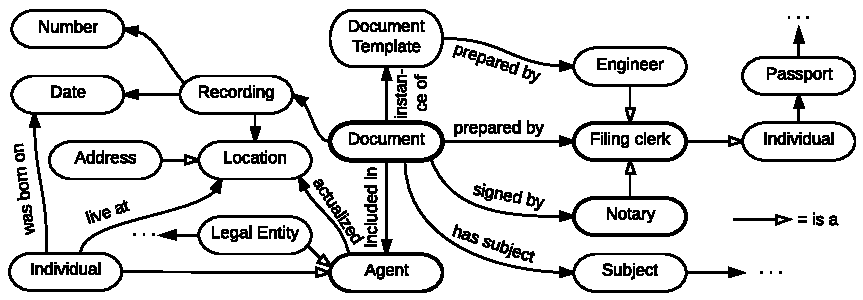
\includegraphics[width=\linewidth]{DocumentOntology-en.pdf}
% where an .eps filename suffix will be assumed under latex,
% and a .pdf suffix will be assumed for pdflatex; or what has been declared
% via \DeclareGraphicsExtensions.
\caption{Upper Layer of Notary Office Ontology}
\label{notaryontology}
\end{figure}

\section{Software Architecture and Implementation}
\label{sec:arch}

The software developed within the project will include two major
versions.  The first one will be a client and server combination,
where client will drive the data mining and visualization procedures,
and server will control storage and access to the graph.  The second
version of the software is a desktop application that is fusion of the
client and server functionality.  The application is intended for
support corporate and personal off-line usage.  The following are the
requirements stated to the software:
\begin{enumerate}
\item the software should be developed as an open-source project,
  this results in possible addition support with a community of
  engineers and users;
\item server software must be not too consumptive to computational and
  memory resources of a shared hosting service; \label{e12:p2}
\item in accordance to \ref{e12:p2}, a support of various database
  back-ends are to be implemented to store triple data.
\end{enumerate}

We orient our efforts in the implementation to a popular hosting
environments that include PHP as programming language and operational
environment, MySQL- and PostgreSQL- servers as a storage, functioning
under Linux operation system.  As a primary client, Firefox web browser
has been chosen and its JavaScript implementation as a client
programming language.

Architecture of the first variant of the software is presented in
fig.~\ref{fig:progsys}.  Server side deal with data storage and
security.  ``Multiformat Storage'' module supports various techniques
of data representation, it could be a SQL-server.  The purpose of
``Data Representation Broker'' module is to convert triples in a
format that is better support special tasks, such as aggregations, and
pass the conversion result to the storage.  In the backward direction,
the broker restores triples from the storage as RDF entities.  In
order to render a template the data model instance should be loaded
through module ``Loader of Triples''.  The instance is represented as
a set of triples.  The security is supplied by “Data Security” module.

At the client side the triples are rendered as HTML tests and combined
into a document by ``Document Renderer'' module.  The result is either
interpreted further by ``RDFa interpreter'' or processed in ``Data
Processing Unit''.  New concepts and relations are sent back to server
as RDF- and RDFa-content.

\noindent\begin{figure}[!t]
\centering
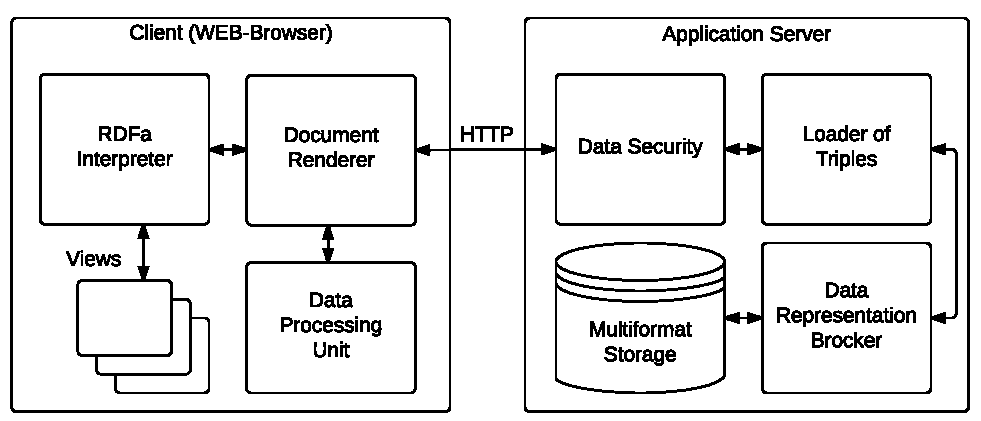
\includegraphics[width=\linewidth]{peixe-architecture-en-2.pdf}
\caption{Program System Architecture}
\label{fig:progsys}
\end{figure}

\subsection{Implementation Software}
\label{sec:implsoft}

Representation of the graph and PHP's access to graph component is
implemented on the base of EasyRdf library.  The library supports
loading RDF-files and represent them as PHP's objects.  The objects
can be accessed in a usual object-oriented way and by means of the
special standard query language SPARQL.

Storing RDF-triples in MySQL is to be implemented with ARC2 library,
which also supports SPARQL-queries.  ARC2 is a development platform
with SW functionality, allowing one to extend the standard set of
routines by means of plug-in modules as well as to create trigger
functions fired as soon as SAPRQL query finished.

Text composition library Zope Page Template (ZPT) is used as a generic
text rendering engine from the logical layer.  ZPT is cross-platform
and allows representing templates and rendering the triples inside.
The templates also stored in RDF.  ZPT technology and its descendants,
like Chameleon, allows programmers and designers to share their common
work on a dynamic HTML page because of ZPT is based on a declarative
approach to template definition.

The engine includes interpreters of several query expression languages
to a logical structures of model and template --- interpreters TAL
(Template Attribute Language) and METAL (Meta TAL).  There are also
tools for internationalization (I18N) support.  Developers of ZPT
successfully solved the following standard web problems:
\begin{IEEEitemize}
\item separation application logic and user interface;
\item utilization of existing HTML-page design software and editors
  (e.g., Dreanweaer) for manipulation of template content with
  conserving TAL and METAL expression;
\item trivial cycle programming structures are replaced with a
  declarative constructions;
\item thanks to METAL templates are manipulated in a powerful manner
  --- cutting and pasting subtrees of a HTML page --- using model data.
\end{IEEEitemize}

To date there are many implementations of TAL and METAL for various
programming systems, including PHP (PHPTAL): the basis syntax and
semantics of TAL does not depend on the implementation language.  For
client-side language JavaScript, ZPT has been implemented by Distal
library, which can also dynamically load model data into rendered
template, resulting consumption more CPU resources of client
workstation and less of server.

The storage module in the desktop application must not be too
consuming the resources of the client workstation, that's why usage of
server software is not particularly expedient, better use in-process
database libraries which are also do not require special configuration
and engineer's attention.  One of the outstanding in-process database
engine is Kyoto Cabinet library \cite{kyoto}, which higher performance
implementation of BerkeleyDB standard.  The library maps blocks of
bytes, i.e. a key to a value, and the mapping is realized by means of
B+-trees and hash tables.  Kyoto Cabinet supports protection against
data loss even due to partial physical damage of hard disks.  The
protection is achieved by special file format and data replication
among a cluster of workstations.

Thus, the nowadays open-source software of internet application
development and relatively cheap server computational resources
completely cover all the requirements of the developing software.


%\subsubsection{Subsubsection Heading Here}
%Subsubsection text here.




% An example of a floating figure using the graphicx package.
% Note that \label must occur AFTER (or within) \caption.
% For figures, \caption should occur after the \includegraphics.
% Note that IEEEtran v1.7 and later has special internal code that
% is designed to preserve the operation of \label within \caption
% even when the captionsoff option is in effect. However, because
% of issues like this, it may be the safest practice to put all your
% \label just after \caption rather than within \caption{}.
%
% Reminder: the "draftcls" or "draftclsnofoot", not "draft", class
% option should be used if it is desired that the figures are to be
% displayed while in draft mode.
%

% Note that IEEE typically puts floats only at the top, even when this
% results in a large percentage of a column being occupied by floats.


% An example of a double column floating figure using two subfigures.
% (The subfig.sty package must be loaded for this to work.)
% The subfigure \label commands are set within each subfloat command, the
% \label for the overall figure must come after \caption.
% \hfil must be used as a separator to get equal spacing.
% The subfigure.sty package works much the same way, except \subfigure is
% used instead of \subfloat.
%
%\begin{figure*}[!t]
%\centerline{\subfloat[Case I]\includegraphics[width=2.5in]{subfigcase1}%
%\label{fig_first_case}}
%\hfil
%\subfloat[Case II]{\includegraphics[width=2.5in]{subfigcase2}%
%\label{fig_second_case}}}
%\caption{Simulation results}
%\label{fig_sim}
%\end{figure*}
%
% Note that often IEEE papers with subfigures do not employ subfigure
% captions (using the optional argument to \subfloat), but instead will
% reference/describe all of them (a), (b), etc., within the main caption.


% An example of a floating table. Note that, for IEEE style tables, the
% \caption command should come BEFORE the table. Table text will default to
% \footnotesize as IEEE normally uses this smaller font for tables.
% The \label must come after \caption as always.
%
%\begin{table}[!t]
%% increase table row spacing, adjust to taste
%\renewcommand{\arraystretch}{1.3}
% if using array.sty, it might be a good idea to tweak the value of
% \extrarowheight as needed to properly center the text within the cells
%\caption{An Example of a Table}
%\label{table_example}
%\centering
%% Some packages, such as MDW tools, offer better commands for making tables
%% than the plain LaTeX2e tabular which is used here.
%\begin{tabular}{|c||c|}
%\hline
%One & Two\\
%\hline
%Three & Four\\
%\hline
%\end{tabular}
%\end{table}


% Note that IEEE does not put floats in the very first column - or typically
% anywhere on the first page for that matter. Also, in-text middle ("here")
% positioning is not used. Most IEEE journals/conferences use top floats
% exclusively. Note that, LaTeX2e, unlike IEEE journals/conferences, places
% footnotes above bottom floats. This can be corrected via the \fnbelowfloat
% command of the stfloats package.



\section{Conclusion}

The research is aimed at support of Semantic Web with algorithms and
software automating text document markup and its logical model
induction.  The approach is based on polysystem representation of the
domain and document content (e.g., web site) as an evolving ontology.
The usage of polysystem of ontologies and the procedure of polysystem
decomposition \cite{father} allows us to solve a number problems in
the activity related to knowledge acquisition in the domain.  New
knowledge are represented as fibers of categories with property of
through cross-fiber interpretation.  In the future, the possibility
will arise for automatic construction of algorithms and programs
implementing a fiber theory in the image and likeness of the known
ones.  At present the polysystem of ontologies allows us to rate and
categorize facts on the domain by analogy with the already known
structures, as well as obtain new interpretations of new concepts
under recognition.

Main part of the paper is devoted to brief description of a technique
of maintenance of an interactive process of the logic model induction
of the document content on the base of data mining of changes of
various versions of the document produced by user.  A problem solution
outline for user dialog conduction aimed at modification and extension
of the logical model with new objects and relations has been
considered.  The dialog is maintained by analyzing and logical
inference in the polysystem representation of the domain ontology.  A
pilot software architecture has been presented as well as brief
overview of used modules and libraries, their properties and feature
has been assessed.

As a testing ground for the technologies under development we decided
to automate a notarial office, where the legal document
representations has both well formalized and unformalized text
fragments.  On the base of the technology a network of document data
exchange can be devised. The security of the document transmission can
be provided as off-line data streams: each physical document is
accompanied with its bar- or QR-code encoding the corresponding
RDF-data of the transferred document. This can result in a semantic
network analogous to nowadays social networks.


% conference papers do not normally have an appendix


% use section* for acknowledgement
\section*{Acknowledgment}
The research is carried on under support of Integration multidisciplinary project of Siberian Branch of Russian Academy of Sciences N 17 “Development of services and infrastructure of scientific spatial data for supporting complex multidisciplinary scientific research of Baikal nature territory”.

%The authors would like to thank...





% trigger a \newpage just before the given reference
% number - used to balance the columns on the last page
% adjust value as needed - may need to be readjusted if
% the document is modified later
%\IEEEtriggeratref{8}
% The "triggered" command can be changed if desired:
%\IEEEtriggercmd{\enlargethispage{-5in}}

% references section

% can use a bibliography generated by BibTeX as a .bbl file
% BibTeX documentation can be easily obtained at:
% http://www.ctan.org/tex-archive/biblio/bibtex/contrib/doc/
% The IEEEtran BibTeX style support page is at:
% http://www.michaelshell.org/tex/ieeetran/bibtex/
%\bibliographystyle{IEEEtran}
% argument is your BibTeX string definitions and bibliography database(s)
%\bibliography{IEEEabrv,../bib/paper}
%
% <OR> manually copy in the resultant .bbl file
% set second argument of \begin to the number of references
% (used to reserve space for the reference number labels box)
\urlstyle{tt}
\begin{thebibliography}{11}
\bibitem{TBL2001} T.~Berners-Lee, J.~Hendler, O.~Lissila. ``The
  Semantic Web A new form of Web content that is meaningful to
  computers will unleash a revolution of new possibilities,''
  Scientific American, May 17, 2001,
  pp.~1-18. URL:~\url{http://sciam.com/article.cfm?articleID=00048144-10D2-1C70-84A9809EC588EF21}
\bibitem{father} A.~K.~Cherkashin. ``Polysystem Analysis and
  Synthesis. Application in Geography,'' Novosibirsk, Russia ``Nauka'' Publ. co.
  1997. -- 502~p. (In Russian)
\bibitem{SN} Social network -- Wikipedia, the free encyclopedia.
  URL:~\url{http://en.wikipedia.org/wiki/Social_network}
\bibitem{prevwork} E.~Cherkashin, P.~Belykh, D.~Annenkov, K.~Paskal, ``A
  Document Content Logical Layer Induction on the Base of Ontologies
  and Processing Changes,'' Procs. of International Conference on
  Applied Internet and Information Technologies, October 25, 2013,
  University of Novi Sad, Technical Faculty ``Mihajlo Pupin'',
  Zrenjanin, Republic of Serbia,
  pp.~252--257. URL:~\url{http://www.tfzr.uns.ac.rs/aiit/archives/AIIT2013/Proceedings.pdf}
\bibitem{b2:15} E.~Cherkashin, V.~Paramonov, et al, ``Model Driven
  Architecture is a Complex System,'' E-Society Journal Research and
  Applications. Volume 2, Number 2, 2011, pp.~15--23.
  URL:~\url{http://www.tfzr.uns.ac.rs/esociety/issues/eSocietyVol2No2.pdf}
\bibitem{b2:5} Model--view--controller --- Wikipedia, the free
  encyclopedia.
  URL:~\url{http://en.wikipedia.org/wiki/Model-view-controller}
\bibitem{zopetal} ``Zope Page Templates Reference,'' The Zope2 Book. URL:~\url{http://docs.zope.org/zope2/zope2book/index.html}
\bibitem{q2} Chameleon -- Chameleon 2.10 documentation.
  URL:~\url{http://chameleon.readthedocs.org/en/latest/}
\bibitem{diff} D.~MacKenzie, P.~Eggert, R.~Stallman. ``Comparing and
  Merging Files,''
  URL:~\url{http://www.gnu.org/software/diffutils/manual/diffutils.pdf}
\bibitem{kyoto} Kyoto Cabinet. URL:~\url{http://fallabs.com/kyotocabinet/}
\end{thebibliography}
% that's all folks
\end{document}
